\chapter{Kajian Pustaka}
\label{chapter:kajian-pustaka}

Bab ini akan diisi oleh kajian pustaka yang berkaitan dengan topik persoalan tugas akhir untuk memberikan informasi mengenai dasar teori dan studi yang dipakai. Bab ini diharapkan dapat membantu pembaca untuk lebih mengerti tentang penelitian tugas akhir ini.

\section{Teknik \textit{Scaling} Basis Data Relasional}

Terdapat berbagai teknik umum yang digunakan untuk melakukan \textit{scaling} pada basis data relasional. Berikut adalah beberapa di antaranya:

\subsection{Replikasi basis data}

Replikasi berarti menyimpan salinan data yang sama pada beberapa mesin yang berbeda dan terhubung melalui jaringan \parencite{dataIntensiveApplications}. Terdapat beberapa alasan mengapa hal ini lazim dilakukan, yaitu:

\begin{enumerate}
    \item Untuk menjaga data tetap dekat secara geografis kepada pengguna, sehingga latensi berkurang.
    \item Agar sistem dapat terus berjalan meski terjadi kegagalan pada sebagian sistem, sehingga \textit{availability} meningkat.
    \item Untuk melakukan \textit{scale out} banyaknya mesin yang bisa melayani \textit{read queries}, sehingga meningkatkan \textit{read throughput}.
\end{enumerate}

Salah satu pendekatan yang umum diimplementasikan pada basis data relasional seperti PostgreSQL adalah replikasi berbasiskan \textit{leader and follower}. Satu \textit{node} ditugaskan sebagai \textit{leader} yang menerima operasi \textit{read and write}, lalu setiap perubahan yang terjadi akan direplikasi oleh replika (\textit{follower}). Dengan pola seperti ini, umumnya operasi \textit{write} hanya dapat ditangani oleh \textit{leader} dan operasi \textit{read} dapat ditangani oleh semua \textit{node}.

\begin{figure}[ht]
    \centering
    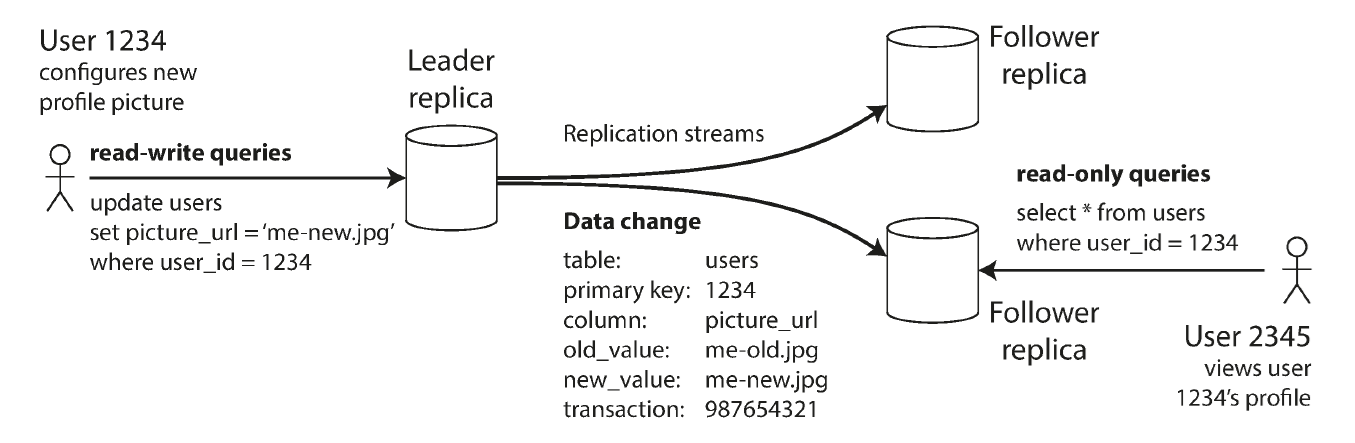
\includegraphics[width=0.8\textwidth]{resources/chapter-2/leader-based-replication.png}
    \caption{\textit{Leader-based (master-slave) replication \parencite{dataIntensiveApplications}}}
    \label{fig:leader-based-replication}
\end{figure}

Selain itu, proses replikasi juga terbagi menjadi dua, yaitu \textit{synchronous replication} dan \textit{asynchronous replication}. Pada \textit{synchronous replication}, data yang akan ditulis juga harus sudah ditulis oleh semua (atau mayoritas) replika sebelum dapat di-\textit{acknowledge}. Pada \textit{asynchronous replication}, data akan ditulis terlebih dahulu pada \textit{leader} lalu perubahannya dipropagasikan kepada \textit{replika}. Setiap pendekatan ini memiliki \textit{tradeoff} tersendiri. \textit{Synchronous replication} menjamin mayoritas \textit{node} memiliki data paling terbaru, tetapi latensi pada proses penulisan akan meningkat, sedangkan pada \textit{asynchronous replication} latensi penulisan jauh lebih kecil, tetapi data pada \textit{replica} menjadi \textit{eventually consistent}. Kedua mode replikasi ini didukung oleh PostgreSQL.

% \section{\textit{The Trends of Unbundling the Database}}

Sebuah \textit{database} terdiri atas beberapa konsep yang digabungkan menjadi satu, yaitu \textit{storage}, \textit{indexing}, \textit{caching}, \textit{query API}, dan terkadang menggabungkannya secara transaksional. \textit{Unbundling the database} berarti memisahkan konsep-konsep tersebut menjadi berbagai layer \parencite{leverageDatabaseInsideOut}.

\subsection{Contoh: \textit{Reinventing Materialized Views}}

Menurut \cite{leverageDatabaseInsideOut}, \textit{materialized views} pada \textit{database}adalah sebuah \textit{query} yang dijalankan \textit{database} lalu disimpan sebagai \textit{cache}. Ketika terdapat perubahan, \textit{materialized view} juga akan diperbarui. Hal ini dilakukan untuk pengoptimalan kinerja. Ketika melakukan \textit{query}, data sudah tersedia lebih awal dan hasil dapat ditampilkan dengan lebih cepat karena \textit{query} tersebut di-\textit{precompute}.

Pendekatan ini sedikit bermasalah karena \textit{materialized view} hanya ada di dalam \textit{database}. Bila konsep ini dikeluarkan dari \textit{database}, kita akan mendapatkan \textit{cache} yang terus menerus diperbarui.

Untuk itu, kita harus menyiapkan tiga hal, yaitu sebuah mekanisme untuk menulis secara transaksional, sebuah \textit{log} yang menyimpan riwayat \textit{writes}, dan \textit{query engine} yang mengubah \textit{log} menjadi \textit{view}.

Berbeda dengan \textit{materialized view}, ketiga hal tersebut bisa dibuat terpisah dan \textit{decentralized} sehingga setiap elemen tersebut beroperasi sebagai entitas yang independen.

\subsection{Keuntungan \textit{Unbundling}}

Salah satu keuntungan terbesar dari \textit{unbundling the database} adalah data tersedia secara \textit{low coupled} sehingga mudah untuk \textit{sharing datasets}. Kemudahan ini berasal dari bentuk sederhana yang diberikan oleh pendekatan \textit{log} yang hanya terdiri atas pembacaan dan penulisan \textit{log} \parencite{leverageDatabaseInsideOut}. Alasan mengapa pendekatan ini umum dipilih akan dijelaskan di bagian berikutnya.

Konsekuensi dari pendekatan ini adalah bahwa sistem tidak harus selalu menyimpan \textit{views}. \textit{View} ini dapat dibuat, dibangun ulang, atau dibuang dengan mudah. Oleh karena itu, \textit{services} didorong untuk hanya mengambil data yang diperlukan saja pada titik waktu tertentu.

% \section{\textit{Append-Only Log}}

\textit{Append-only log} merupakan sebuah pendekatan alternatif yang bisa diambil untuk menyederhanakan masalah yang ditimbulkan karena teorema CAP. Ide dasarnya adalah dengan menghilangkan operasi \textit{update} dan \textit{delete} pada CRUD, sehingga menyisakan \textit{read} dan \textit{create} \parencite{howToBeatCAP}.

\subsection{\textit{Rethinking Data System}}

Aplikasi data terdiri atas berbagai hal, mulai dari penyimpanan data, pengambilan data, \textit{joins}, agregasi, \textit{stream processing}, dan lain-lain. Meskipun begitu, hal tersebut bisa disederhanakan menjadi hal berikut.

\[Query = Function(All Data)\]

Sebuah \textit{data system} menjawab pertanyaan atas sebuah \textit{dataset}. Pertanyaan tersebut dinamakan sebagai \textit{queries}. Persamaan di atas menyatakan bahwa \textit{query} merupakan fungsi pada keseluruhan data yang dimiliki.

Menurut \cite{howToBeatCAP}, \textit{A piece of data is an indivisible unit that you hold to be true for no other reason that it exists}. Terdapat dua \textit{properties} yang dimiliki data. Pertama, data terikat pada waktu. Sebuah data adalah fakta yang diketahui benar pada satu titik waktu tertentu. Kedua, data pada dasarnya \textit{immutable}. Karena hubungannya dengan waktu, kebenaran sebuah data tidak berubah. Misalkan, Budi tinggal di Bandung. Setelahnya, Budi tinggal di Jakarta. Data terbaru yang menyatakan bahwa Budi tinggal di Jakarta tidak lantas membuat fakta bahwa Budi (pernah) tinggal di Bandung salah.

Operasi \textit{update} bisa dihilangkan karena tidak logis dalam konteks \textit{immutable data}. Misalnya, men-\textit{update} lokasi Budi berarti bahwa kita menambahkan data lokasi Budi yang lebih baru.

Operasi \textit{delete} bisa dihilangkan karena operasi ini juga dapat direpresentasikan dengan data baru. Misalkan, bila Upin berhenti mengikuti Ipin di sosial media, hal tersebut tidak mengubah fakta bahwa Upin pernah mengikuti Ipin. Hanya saja, Upin berhenti mengikuti Ipin pada titik waktu tertentu.

Konsep kedua adalah \textit{query}. \textit{Query} adalah turunan dari data. Misalkan pertanyaan "Di mana lokasi Budi sekarang?" merupakan sebuah \textit{query}. \textit{Query} ini dapat diturunkan dengan mengembalikan data terakhir yang berkaitan dengan lokasi Budi.

\subsection{\textit{Beating CAP Theorem}}



\subsection{\textit{Event Sourcing} dan \textit{Change Data Capture}}

Menurut \cite{dataIntensiveApplications}, \textit{change data capture (CDC)} merupakan sebuah proses yang mengobservasi setiap perubahan pada data yang ditulis ke dalam basis data dan mengekstraknya ke dalam bentuk yang bisa direplikasi oleh sistem lain. Sebagai contoh, perubahan pada database bisa di-\textit{capture} lalu diterapkan pada \textit{search index} untuk menyamakan data pada basis data. Apabila \textit{log} diaplikasikan dalam urutan yang sama, data pada \textit{search index} dan basis data bisa dipastikan sama.

Mirip seperti \textit{change data capture}, \textit{event sourcing} juga menyimpan setiap perubahan pada \textit{state} aplikasi sebagai \textit{log of events}. Perbedaan terbesarnya terletak pada level abstraksinya. Pada \textit{change data capture}, aplikasi menggunakan basis data \textit{in a mutable way} dan dapat memperbarui atau menghapus \textit{record} sesuka hati. Aplikasi yang menulis pada basis data tidak harus \textit{aware} bahwa terdapat CDC. Berbeda dengan \textit{event sourcing}, logika aplikasi dibandung secara eksplisit di atas asumsi \textit{immutable event} yang ditulis pada \textit{event log}. Pada kasus ini, \textit{event} berupa \textit{append only}. Singkatnya, \textit{event sourcing} didesain untuk bisa merefleksikan hal yang terjadi pada level aplikasi dan bukan pada \textit{low-level state changes}.

% \section{\textit{Stateful Real-Time Stream Processing}}

\subsection{\textit{Stream Processing}}

Secara umum, \textit{stream} merujuk pada data yang tersedia secara inkremental dari waktu ke waktu. Konsep ini dipakai di berbagai tempat, seperti stdin dan stdout Unix, TCP \textit{connection}, dan lain-lain \parencite{dataIntensiveApplications}.

\textit{Stream processing} merupakan paradigma pemrograman yang memandang \textit{streams} atau urutan \textit{events} sebagai objek \textit{input} dan \textit{output} utama dari komputasi. \cite{streaming101} menyatakan bahwa \textit{stream processing} merupakan tipe \textit{engine} pemrosesan data yang didesain dengan mempertimbangkan \textit{dataset} yang tidak terbatas.

\cite{streamProcessingComparison} menyatakan bahwa terdapat karakteristik penting pada \textit{stream processing}, yaitu:

\begin{enumerate}
    \item \textit{Delivery guarantees}. Setiap informasi yang masuk harus dijamin akan diproses oleh \textit{streaming engine}.
    \item \textit{Fault tolerance}. Ketika terjadi kegagalan, \textit{streaming engine} harus mampu melakukan \textit{recovery} dan memulai ulang dari titik yang ditinggalkan.
    \item \textit{State management}. \textit{Streaming engine} harus memiliki mekanisme untuk menyimpan dan memperbarui informasi \textit{state}.
    \item Memiliki kinerja yang baik dari sisi latensi, \textit{throughput}, dan \textit{scalability}.
    \item Memiliki fitur yang lebih \textit{advances}, seperti \textit{event time processing}, \textit{watermarks}, \textit{windowing}, dan lain-lain.
\end{enumerate}

Selain itu, karakteristik \textit{stream processing} juga bisa dibagi menjadi dua jenis, yaitu:

\begin{enumerate}
    \item \textit{Native streaming}. \textit{Stream processing} jenis ini akan langsung memproses \textit{record} yang diterima secepat mungkin. Contoh \textit{stream processing} tipe ini adalah Apache Storm, Apache Flink, Apache Kafka Streams, dan Apache Samza.
    \item \textit{Micro-batching}. \textit{Stream processing} jenis ini meproses \textit{record} setiap beberapa detik atau milidetik sekali sehingga \textit{record} diproses dalam setiap \textit{mini-batch} dengan sedikit \textit{delay}. Contoh \textit{stream processing} tipe ini adalah Apahe Spark Streaming dan Apache Storm-Trident.
\end{enumerate}

% \section{\textit{Deployment Plan}}

\textit{Deployment plan} adalah pemetaan antara sistem, \textit{software}, dan deployment, yang dapat dikaitkan dengan data untuk konfigurasi serta \textit{dependency} dari masing masing bagian dan alasan untuk melakukan \textit{deployment} \parencite{ARCANGELI2015198}.

% \section{Kubernetes}

Kubernetes adalah sebuah solusi \textit{open source} yang berguna untuk melakukan orkestrasi berbagai aplikasi yang telah dibungkus dalam suatu lingkungan yang disebut sebagai \textit{container}. Kubernetes berfungsi untuk melakukan \textit{deployment} otomatis, \textit{auto scaling} secara otomatis, serta membuat \textit{network} untuk menghubungkan \textit{container} dengan \textit{container} lainnya. Kubernetes membantu mengelola dan mempercepat proses pengembangan layanan yang rumit dengan skala yang besar \parencite{helmkubernetes}.

Kubernetes memiliki beberapa komponen yang digunakan ketika mengelola layanan. \textit{Node, pod, service} dan \textit{deployment} merupakan empat komponen utama yang sering kali menjadi komponen utama ketika membuat suatu layanan dengan Kubernetes. \textit{Node} dapat dianalogikan dengan lingkungan \textit{virtual machine} yang memiliki kemampuan terbatas. \textit{Pod} merupakan suatu tempat untuk menjalankan berbagai macam \textit{container} di dalamnya. Satu \textit{pod} dapat memiliki lebih dari satu \textit{container} untuk dioperasikan. \textit{Service} berfungsi untuk membuka akses eksternal ke dalam \textit{pod} yang secara umum bersifat internal dan tidak dapat diakses dari luar. Terakhir, yaitu \textit{deployment} adalah suatu konfigurasi untuk menjalankan layanan yang akan dibuat, konfigurasi \textit{deployment} juga melingkupi komponen \textit{pod} dan \textit{service}.

Kubernetes memiliki fitur seperti \textit{auto scaling, self-healing, device discovery, load balancing} serta \textit{rollout} dan \textit{rollback}. \textit{Auto scaling} sering digunakan untuk menjaga sistem untuk terus beroperasi dengan cara melakukan replikasi layanan dengan jumlah yang ditentukan. \textit{Self healing} memastikan bahwa layanan yang sedang mengalami kegagalan dapat diperbaiki secara otomatis. \textit{Rollout} dan \textit{Rollback} sering digunakan ketika melakukan proses \textit{deployment} untuk mencegah adanya \textit{downtime} ketika meluncurkan layanan versi baru. Seluruh fitur yang disebutkan bekerja sama untuk membuat kubernetes dapat mengelola aplikasi dalam skala yang masif dan mempertahankan kualitas layanan yang dibuat.

\subsection{\textit{Pod component}}

\textit{Pod} merupakan abstraksi unit atau komponen terkecil pada Kubernetes untuk memudahkan proses pengembangan. \textit{Pod} merupakan sebuah lingkunan linux yang digunakan secara bersama namun memiliki sumber daya yang terpisah dan terbatas melalui teknologi linux cgroups dan namespace untuk menjalankan satu atau lebih \textit{container}. \textit{Pod} bersifat \textit{ephemeral} sehingga seluruh sumber daya akan hilang apabila \textit{pod} mengalami kegagalan \parencite{pod}.

Untuk memastikan bahwa layanan dapat selalu berjalan dengan baik, semua kegiatan yang berkaitan dengan \textit{pod} mulai dari \textit{scaling} hingga \textit{health check} akan dilakukan oleh Kubernetes. Kubernetes akan bertanggung jawab untuk melakukan \textit{penjadwalan} serta pencocokan konfigurasi maupun siklus hidup dari \textit{pod} tersebut. Dengan abstraksi \textit{pod}, proses pengembangan layanan menggunakan Kubernetes semakin mudah untuk dipahami dan dilakukan.

\subsection{\textit{Service component}}

Service merupakan suatu abstraksi untuk membuat \textit{pod} dapat diakses secara eksternal. \textit{Pod} bersifat dan \textit{ephemeral} dan tidak dapat diakses dari luar \textit{pod}. Melalui abstraksi \textit{service} Kubernetes, \textit{pod} tersebut dapat diakses secara eksternal dengan cara membuat suatu layanan intermediet untuk meneruskan \textit{request} dari eksternal.
Layanan intermediet yang disediakan oleh \textit{service} diantaranya \textit{ClusterIp, NodePort, LoadBalancer} dan  \textit{ExternalName}.

ClusterIP bersifat internal dan sangat berkaitan erat dengan \textit{pod}. Apabila \textit{service} tidak dibuat konfigurasinya, \textit{pod} akan selalu memiliki \textit{service} dengan tipe \textit{ClusterIP}. \textit{NodePort} dan \textit{LoadBalancer} akan membuat \textit{pod} dapat ditemukan oleh layanan eksternal dan diakses melalui perangkat lain. Kedua tipe tersebut akan membuat sebuah \textit{endpoint} untuk meneruskan \textit{request} yang masuk berdasarkan label yang diletakan ketika membuat \textit{pod} \parencite{service}.
\subsection{\textit{Deployment component}}

\textit{Deployment} merupakan abstraksi yang menggabungkan kedua abstraksi \textit{pod} dan \textit{service}. \textit{Deployment} dapat melihat kondisi seluruh sistem pada saat keadaan awal maupun keadaan berubah. \textit{Deployment} akan menyimpan keadaan sistem secara berkala dan melakukan pengecekan secara deklaratif untuk mendeteksi perubahan keadaan sistem saat ini dengan keadaan sistem yang diinginkan \parencite{deployment}.

\textit{Deployment} memiliki fitur \textit{rollout} dan \textit{rollback} untuk meningkatkan \textit{availability} layanan. \textit{Rollback} menurunkan versi dari layanan yang saat ini sedang berjalan sedangkan \textit{rollout} melakukan \textit{upgrade} layanan. Kedua fitur ini berjalan dengan cara membuat \textit{replica} dari layanan yang sedang berjalan untuk mencegah penurunan \textit{availability}. Ketika \textit{deployment} ingin menaikkan versi layanan yang digunakan, \textit{deployment} akan membuat \textit{pods} dengan versi terbaru. Ketika \textit{pods} ini sudah aktif beroperasi serta memiliki status \textit{healthy}, layanan dengan versi sebelumnya baru bisa dihapus \parencite{deployment}.

% Node merupakan suatu lingkungan terisolasi yang menjadi komponen dasar dalam pengelolaan aplikasi dengan kubernetes. 

% \section{Kubernetes distribution}
Dalam penelitian ini akan dibahas tiga distribusi Kubernetes, yaitu KubeEdge, MicroK8s, serta K3s. Masing masing dari distribusi ini memiliki kegunaan dan fungsi nya masing masing. Walaupun semuanya memiliki \textit{support} untuk IoT namun setiap distribusi memiliki cara unik tersendiri untuk menyelesaikan masalahnya.

\subsection{KubeEdge}
KubeEdge merupakan solusi \textit{edge architecture} \textit{open source} yang mengembangkan Kubernetes secara lebih jauh untuk domain spesifik yaitu IoT \parencite{kubeedge}. Arsitektur KubeEdge memungkinkan untuk melakukan konfigurasi perangkat IoT yang berada di \textit{edge} secara terpusat melalui komponen \textit{cloud}. Dengan adanya dua komponen \textit{edge core} dan \textit{cloud core}, komunikasi antara platform aplikasi menjadi \textit{seamless}.

Untuk menghubungkan \textit{cloud core} dengan \textit{edge core}, KubeEdge menggunakan sebuah \textit{controller} yang dapat melakukan \textit{device discovery} terhadap \textit{edge core}. Setelah \textit{edge core} ditemukan, \textit{controller} akan meneruskan \textit{request} ke komponen berikutnya yaitu \textit{Sync Service}. KubeEdge menggunakan KubeBus untuk melakukan komunikasi antara \textit{cloud} dan \textit{edge}, KubeBus menggunakan protokol HTTP untuk meneruskan \textit{request} dari \textit{cloud core} menuju \textit{edge core}. Setelah \textit{request} diterima oleh \textit{edge core}, akan digunakan protokol MQTT untuk menerima ataupun mengirim data dari perangkat IoT ke \textit{edge core} dan juga sebaliknya. Ilustrasi arsitektur dapat dilihat pada gambar \ref*{fig:arsitektur-kube-edge}.

\begin{figure}[ht]
  \centering
  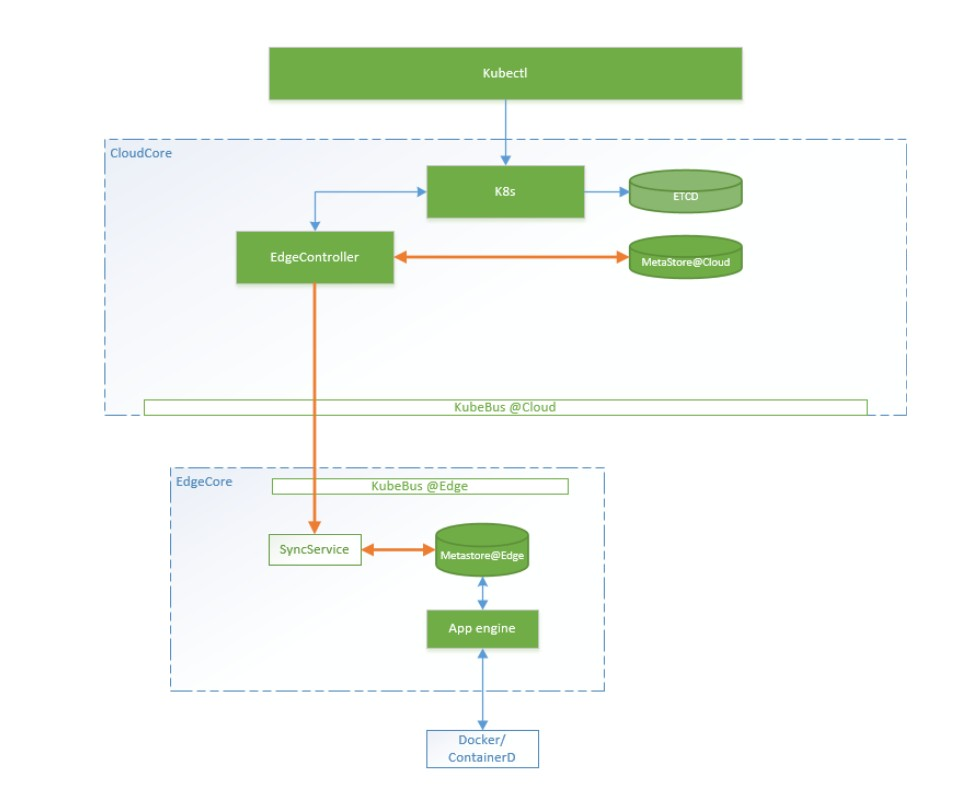
\includegraphics[width=0.5\textwidth]{resources/chapter-2/arsitektur-kube-edge.jpg}
  \caption{Arsitektur KubeEdge \parencite{kubeedge}}
  \label{fig:arsitektur-kube-edge}
\end{figure}

\subsection{Microk8s}
MicroK8s adalah sebuah platform \textit{open-source} yang digunakan untuk mengotomatisasi distribusi, \textit{scaling}, dan manajemen aplikasi yang berbasis kontainer. MicroK8s menyediakan fungsionalitas inti pada Kubernetes, dengan ukuran yang kecil, dan dapat di-\textit{scale} dari satu node hingga menjadi kluster produksi yang besar \parencite{microk8s}.

Dengan mengurangi penggunaan sumber daya yang dibutuhkan untuk menjalankan Kubernetes, MicroK8s memungkinkan penggunaan Kubernetes dalam berbagai lingkungan, seperti:

\begin{enumerate}
  \item Mengubah Kubernetes menjadi alat pengembangan yang ringan.
  \item Menjadikan Kubernetes tersedia untuk digunakan dalam lingkungan minimal seperti GitHub CI (Continuous Integration).
  \item Menyesuaikan Kubernetes untuk aplikasi IoT pada perangkat dengan sumber daya terbatas.
\end{enumerate}


\subsection{K3s}
K3s adalah sebuah platform \textit{open-source} yang memfasilitasi penggunaan Kubernetes dengan ukuran yang lebih ringan dan mudah diimplementasikan. K3s dikembangkan untuk memudahkan distribusi dan manajemen Kubernetes dalam lingkungan yang lebih sederhana dan bersifat minimalis. K3s dibuat untuk mendukung pengembangan pada ranah IoT karena K3s memiliki dukungan sepenuhnya untuk arsitektur ARM serta cocok untuk digunakan pada lingkungan \textit{edge} dan IoT \parencite{k3s}.

K3s memiliki dua komponen utama, yaitu \textit{server} dan \textit{agent}. \textit{Server} dapat dikatakan sebagai sebuah \textit{control plane} atau \textit{master node} yang digunakan pada K3s dan berfungsi untuk mengatur seluruh permintaan ataupun \textit{request} dari \textit{agent}. \textit{Server} memiliki tanggung jawab penuh terhadap masing masing \textit{agent} yang terhubung mulai dari menyimpan data dari masing masing \textit{agent}, \textit{controller}, serta \textit{scheduler} \parencite{k3s}. Di sisi lain, \textit{agent} berfungsi sebagai \textit{slave node} yang akan mengeksekusi semua perintah dari \textit{server} atau \textit{master node}. Ilustrasi arsitektur dapat dilihat pada gambar \ref{fig:arsitektur-k3s}.

\begin{figure}[ht]
  \centering
  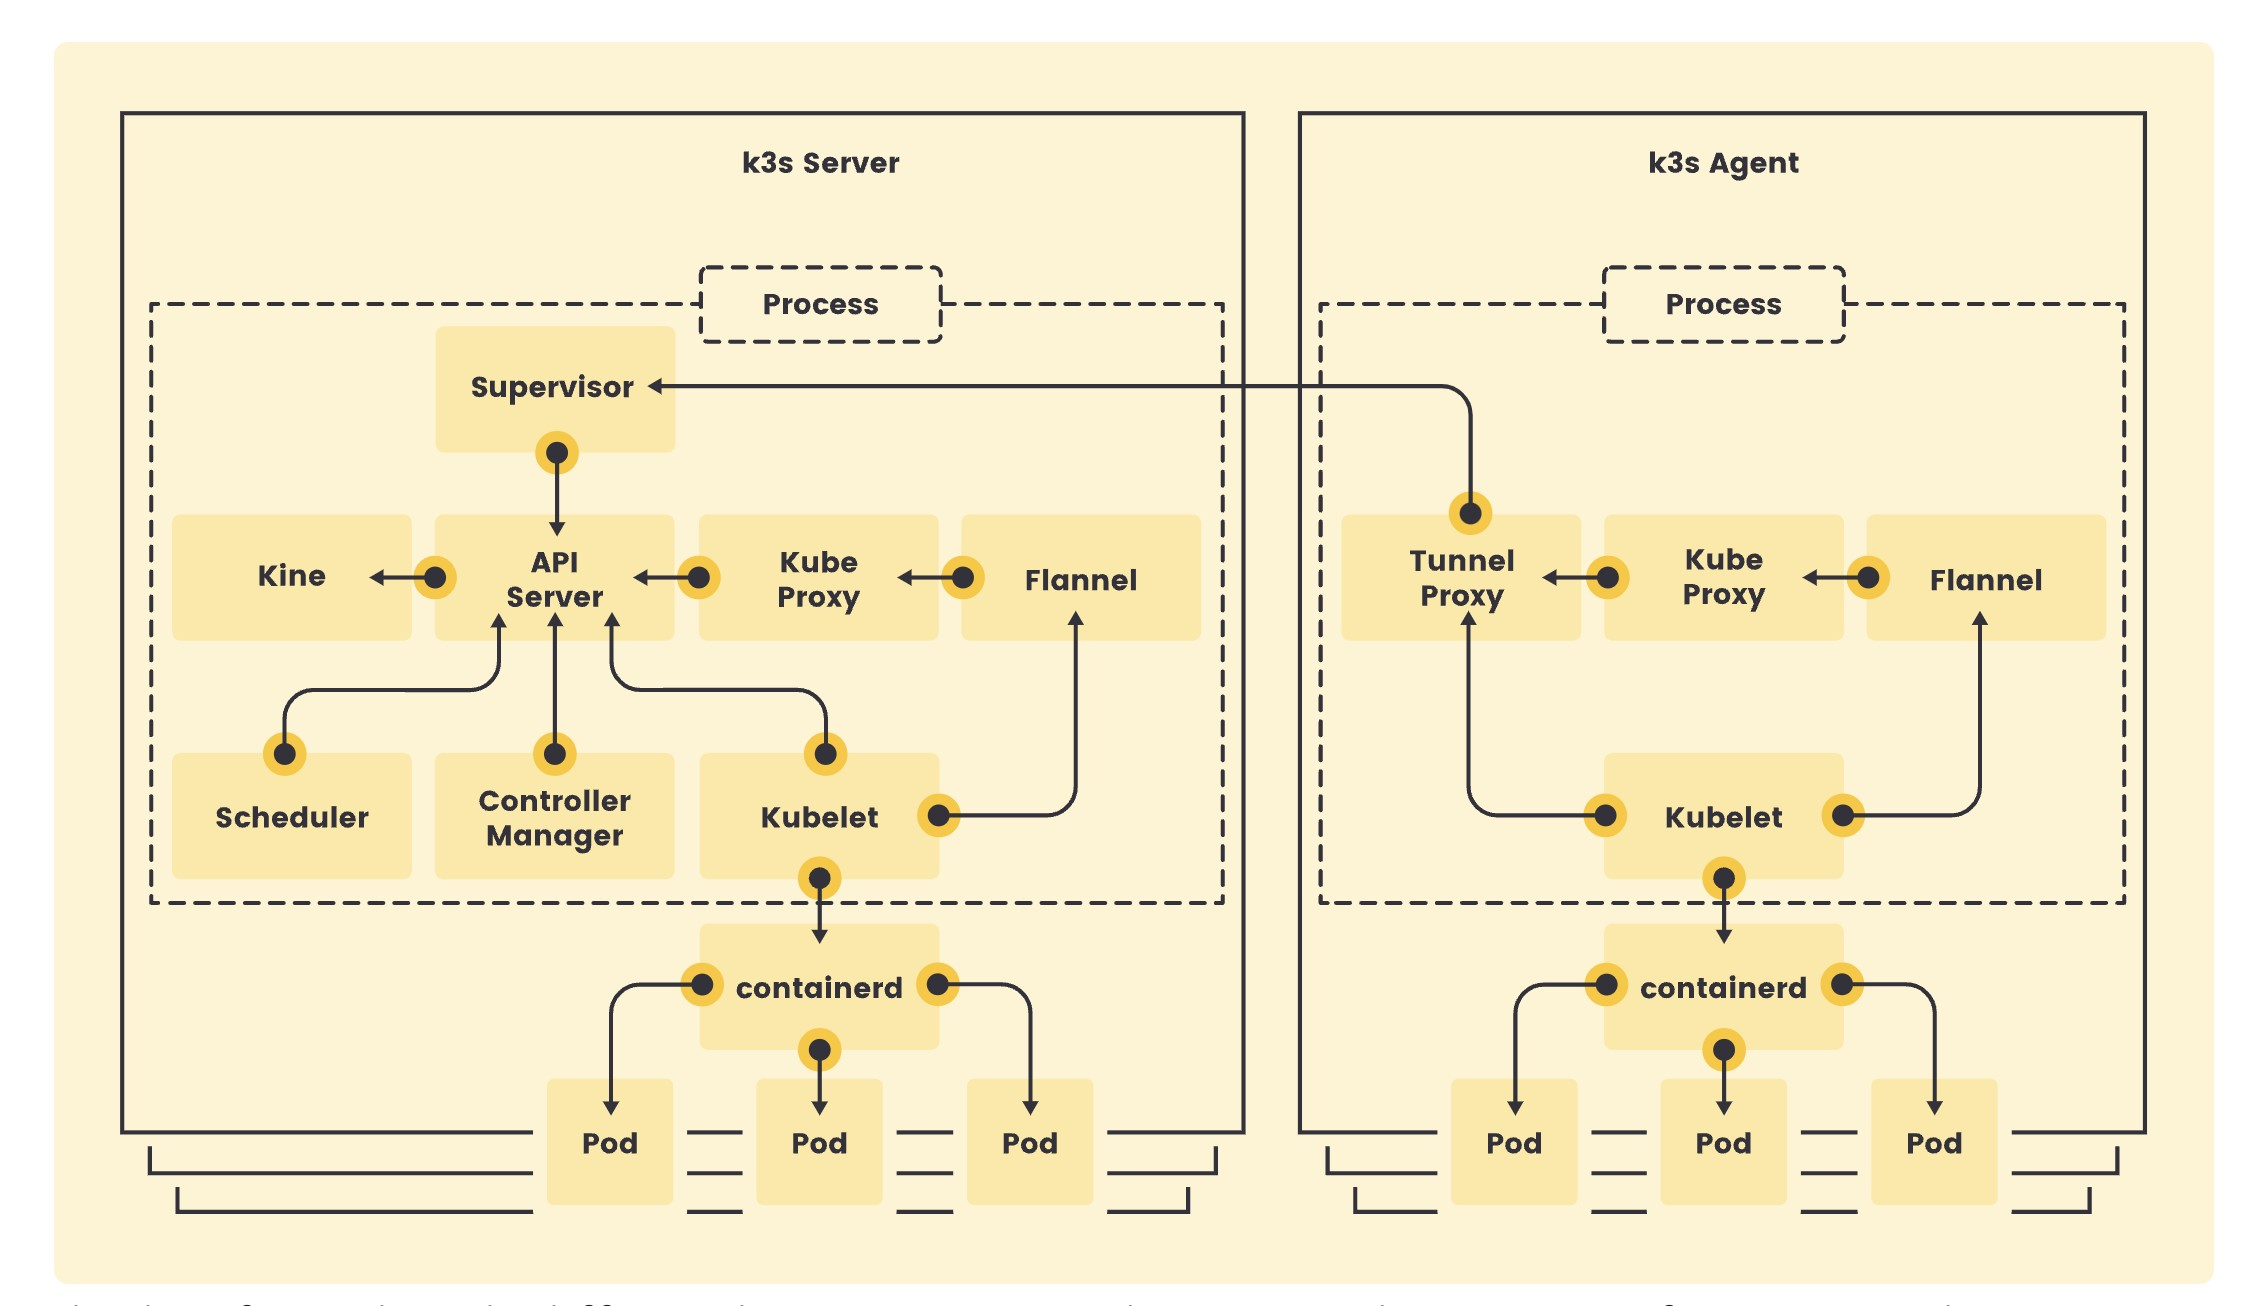
\includegraphics[width=1\textwidth]{resources/chapter-2/arsitektur-k3s.jpg}
  \caption{Arsitektur K3s \parencite{k3s}}
  \label{fig:arsitektur-k3s}
\end{figure}

\pagebreak

% \section{IoT}



\textit{Internet of Things (IoT)} adalah sebuah infrastruktur dari objek, orang, sistem, serta sumber daya informasi yang saling terhubung dengan layanan cerdas untuk memproses informasi dari dunia fisik dan virtual \parencite{Dias2019}. Konsep dan paradigma \textit{Internet of Things} ini merupakan perwujudan dari evolusi teknologi informasi karena dapat membuat kehidupan menjadi lebih baik dalam berbagai sektor. Setiap objek yang ditemukan pada kegiatan sehari-hari, bertransformasi menjadi entitas cerdas yang mampu berinteraksi dengan lingkungan sekitarnya dan jaringan digital secara lebih luas. IoT memperkenalkan kemungkinan baru dalam otomatisasi dan pengambilan keputusan yang berbasis data, membuka jalan bagi inovasi lintas sektor \parencite{madakam2015internet}.

\begin{figure}[ht]
  \centering
  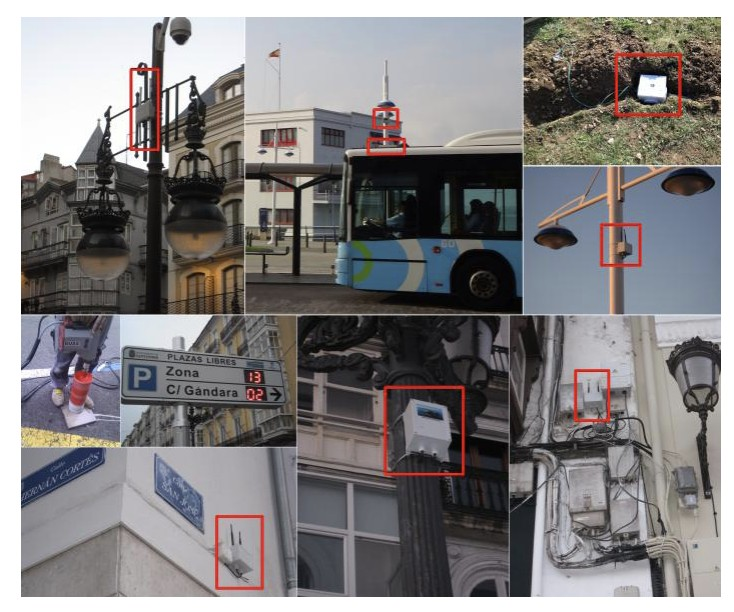
\includegraphics[width=0.8\textwidth]{resources/chapter-2/gambar-iot.jpg}
  \caption{Perangkat IoT yang Terdapat pada Lingkungan Sekitar \parencite{sotres2017practical}}
  \label{fig:iot-kehidupan-sehari-hari}
\end{figure}

IoT memiliki aplikasi yang luas di berbagai sektor, termasuk industri, kesehatan, transportasi, dan pertanian. Dalam sektor industri, IoT memungkinkan otomatisasi proses dan pemantauan efisiensi mesin secara real-time. Di bidang kesehatan, IoT berkontribusi pada pengembangan perangkat medis yang terhubung untuk pemantauan kesehatan pasien. Dalam transportasi, IoT mendukung pengembangan kendaraan otonom dan sistem manajemen lalu lintas cerdas. Di sektor pertanian, IoT digunakan untuk memantau kondisi tanah dan iklim, membantu petani dalam pengambilan keputusan seperti pada gambar \ref{fig:iot-kehidupan-sehari-hari}

IoT dapat dibagi menjadi tiga lapisan, yaitu lapisan persepsi, lapisan jaringan, dan lapisan aplikasi secara berurutan. Lapisan persepsi bertanggung jawab atas pengumpulan data dalam IoT. Lapisan ini terdiri dari berbagai jenis sensor, seperti sensor suhu, sensor kelembaban, RFID, kamera, GPS, dan sebagainya. Lapisan jaringan terdiri dari berbagai jenis jaringan, seperti internet, jaringan komunikasi 2G dan 3G, serta jaringan siaran. Lapisan jaringan terutama digunakan untuk mengumpulkan data dari lapisan persepsi dan memproses data tersebut untuk lapisan aplikasi. Lapisan terakhir, yaitu lapisan aplikasi, adalah antarmuka antara pengguna dan IoT. Banyak aplikasi, termasuk logistik, rantai pasokan, pertanian, industri, keamanan publik, pengelolaan perkotaan, telemedis, rumah pintar, transportasi pintar, dan pemantauan lingkungan, diaktifkan melalui IoT \parencite{SmartHomeSystemBasedOnIoTTechnologies}. Tidak hanya itu, kemunculan berbagai perangkat IoT baru yang memerlukan \textit{update} secara berkala juga menimbulkan masalah baru yakni sulitnya melakukan \textit{update} untuk setiap perangkat yang ada apabila jumlahnya semakin meningkat sehingga peran \textit{remote deployment} menjadi sangat penting dalam menyelesaikan masalah ini \parencite{RemoteDeployment}.

% \section{\textit{Service}}

\textit{Service} dapat diartikan sebagai sebuah teknologi atau cara kerja yang dapat digunakan untuk memberikan keuntungan ataupun menyelesaikan suatu pekerjaan. Selain itu \textit{service} juga dapat diartikan sebagai abstraksi dari sebuah proses bisnis. \parencite{osullivan2002}

Secara umum \textit{Service} Memiliki tiga fitur utama yaitu.
\begin{enumerate}
  \item \textit{Service} dapat melakukan sebuah aksi atau pekerjaan untuk orang lain,
  \item \textit{Service} adalah sebuah aset yang memiliki sebuah nilai yang dapat diturunkan dari penyedia ke pengguna,
  \item \textit{Service} dapat di bungkus pada service lainnya (sub-services),
\end{enumerate}

Untuk menggabungkan \textit{service}, terdapat dua cara yaitu agregasi dan komposisi. Agregasi memiliki pendekatan untuk menggabungkan dua atau lebih \textit{service} dan membuat satu \textit{entrypoint} untuk seluruh \textit{service} tersebut. Berbeda dengan komposisi, komposisi menggunakan pendekatan untuk mengintegrasikan seluruh sub-\textit{services} yang ada dengan cara membuat jalur komunikasi antar \textit{service} dan setiap \textit{service} memiliki hubungan tertentu dengan \textit{service} lainnya.

Interaksi pada sebuah \textit{service} haruslah minimal memiliki tiga elemen, \textit{service provider}, \textit{service requestor/client}, serta \textit{\textit{service registry}}, namun terdapat juga elemen ke empat pada beberapa kasus yaitu \textit{service broker}. Ilustrasi dapat dilhat pada gambar \ref{fig:tiga-elemen-service}

\begin{figure}[ht]
  \centering
  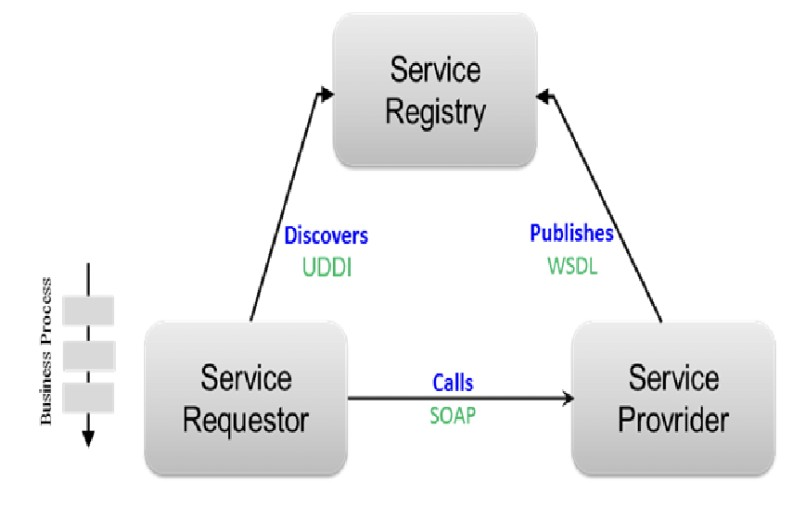
\includegraphics[width=0.8\textwidth]{chapter-2/tiga-elemen-service.jpg}
  \caption{Tiga Elemen pada Interaksi Service, \parencite{abugessaisa2023}}
  \label{fig:tiga-elemen-service}
\end{figure}

\textit{Service requestor} mengirimkan permintaannya serta kebutuhannya kepada \textit{service registry} untuk dicarikan service yang sesuai dengan kebutuhannya. Namun pada beberapa kasus khusus, \textit{service requestor}
sudah memiliki \textquotedblleft contract \textquotedblright dengan \textit{provider} tujuannya sehingga bisa langsung melakukan \textit{request} ke \textit{provider} tanpa bantuan dari \textit{service registry}.

Service \textit{provider} menyediakan \textit{service} yang dapat dikonsumsi oleh publik, agar \textit{service} nya dapat digunakan oleh requestor, \textit{service} \textit{provider} akan memberikan list \textit{services} yang dimiliki kepada registry untuk disimpan pada sebuah \textquotedblleft catalogue \textquotedblright yang dimiliki oleh registry.\textit{Service registry} berperan sebagai penengah dalam komunikasi \textit{requestor} dan \textit{provider}. \textit{Service registry} memiliki \textquotedblleft catalogue \textquotedblright yang menyimpan list berbagai macam \textit{service provider} yang dapat digunakan oleh \textit{service requestor}.

Dengan adanya ketiga elemen tersebut, interaksi pada \textit{services} dapat berjalan sehingga menciptakan suatu fungsionalitas seperti proses bisnis ataupun pemenuhan kebutuhan lainnya.


% \section{\textit{Service discovery}}

\textit{Service discovery} adalah proses mencari layanan yang tersedia dan relevan untuk permintaan tertentu berdasarkan deskripsi semantik fungsional dan non-fungsional. \parencite{klusch2014servicediscovery}. \textit{Servie discovery} merupakan masalah yang sangat penting untuk menyelesaikan masalah konfigurasi. \textit{Service discovery} memungkinkan perangkat dan layanan untuk saling menemukan satu sama lain, mengatur diri, dan berkomunikasi dengan lancar. Namun, seringkali \textit{service discovery} tidak dimanfaatkan secara baik sehingga menghabiskan waktu untuk mencari layanan secara aktif dan mengatur perangkat dan program secara manual. Terkadang, konfigurasi layanan memerlukan keahlian khusus lainnya yang tidak berhubungan dengan apa yang ingin dicapai, sehingga hal ini membuat proses menjadi terhambat. Service discovery membantu untuk mengatasi masalah ini dengan membuat proses ini lebih otomatis dan mudah dilakukan \parencite{ServiceDiscovery}.

Dalam pengaplikasiannya terdapat beberapa \textit{pattern} yang dapat diaplikasikan dalam implementasi \textit{service discovery}. Menurut \parencite{micoservicearchitecture}, terdapat lima \textit{pattern} yang dapat digunakan ketika mengimplementasikan \textit{service discovery} yaitu \textit{3rd Party Registration, Client Side Serivce, Self Registration, serta Server-side service discovery}. Masing masing \textit{pattern} memiliki keunggulan dan kegunaan khusus sehingga perlu dipahami fungsi dari setiap \textit{pattern}.

\subsection{\textit{3rd Party Registration}}
\textit{3rd Party Registration pattern} adalah solusi yang digunakan pada kasus ketika service dapat di-\textit{register} dan \textit{unregister} pada \textit{registar} atau \textit{provider} nya. Solusi ini mewajibkan untuk melakukan registrasi kepada \textit{registar} ketika layanan baru dinyalakan dan melakukan \textit{unregister} ketika layanan dimatikan. layanan \textit{3rd party} yang bertanggung jawab sebagai \textit{registar} untuk mengelola hal ini \parencite{3rdpartyintegration}. Beberapa \textit{tools} yang telah menyediakan sistem layanan seperti ini yaitu \textit{Netflix Prana} yang akan bertindak sebagai \textit{side car} untuk aplikasi non-\textit{JVM} seperti Eureka ataupun AWS \textit{autoscaling groups} yang akan secara otomatis untuk meregister dan menghilangkan EC2 instance pada \textit{load balancer} nya.

Keuntungan untuk menggunakan \textit{pattern} ini ialah proses pembuatan kode yang mudah karena bergantung kepada \textit{3rd party} untuk proses registrasinya. Serta layanan \textit{3rd party} pun akan bertanggung jawab untuk melakukan pengecekan secara berkala agar sistem terus aktif sehingga meningkatkan \textit{availabilty} sistem. Namun, terdapat beberapa kekurangan diantaranya layanan \textit{3rd party} ini hanya bisa untuk melakukan \textit{discovery} secara umum. Seringkali dibutuhkan suatu solusi spesifik yang menjawab permasalahan khusus yang tidak bisa hanya diselesaikan dengan solusi seperti ini, perlu dibuat solusi \textit{custom} yang dapat menambah komponen baru ataupun arsitektur lain yang dapat menyelesaikan masalah tersebut \parencite{3rdpartyintegration}.

\subsection{\textit{Client Side}}
\textit{Client Side pattern} adalah suatu solusi \textit{service discovery} dengan proses \textit{client} yang mencari lokasi \textit{service} yang ingin dituju. \textit{Client} akan mencari lokasi dari tujuan dengan cara melakukan \textit{query} ke \textit{service registry} sehingga lokasi dari \textit{service} yang dituju dapat ditemukan secara dinamis dan \textit{runtime}. Beberapa keunggulan dari \textit{pattern} ini adalah mengurangi kompleksitas dan latensi karena mengurangi jumlah \textit{node} yang perlu di kunjungi. Namun salah satu kekurangannya yaitu meningkatnya kompleksitas kode yang dibuat, karena proses pencarian \textit{service} diletakkan di \textit{client} maka proses pencarian dan perubahan sepenuhnya dibebankan pada \textit{client}. Hal ini membuat proses pencarian tidak \textit{scalable} dan sulit ketika akan melakukan perubahan \parencite{clientsidediscovery}. Visualisasi dari \textit{client side service discovery} dapat dilihat pada \textbf{Gambar \ref{fig:client-side-discovery}}

\begin{figure}[ht]
  \centering
  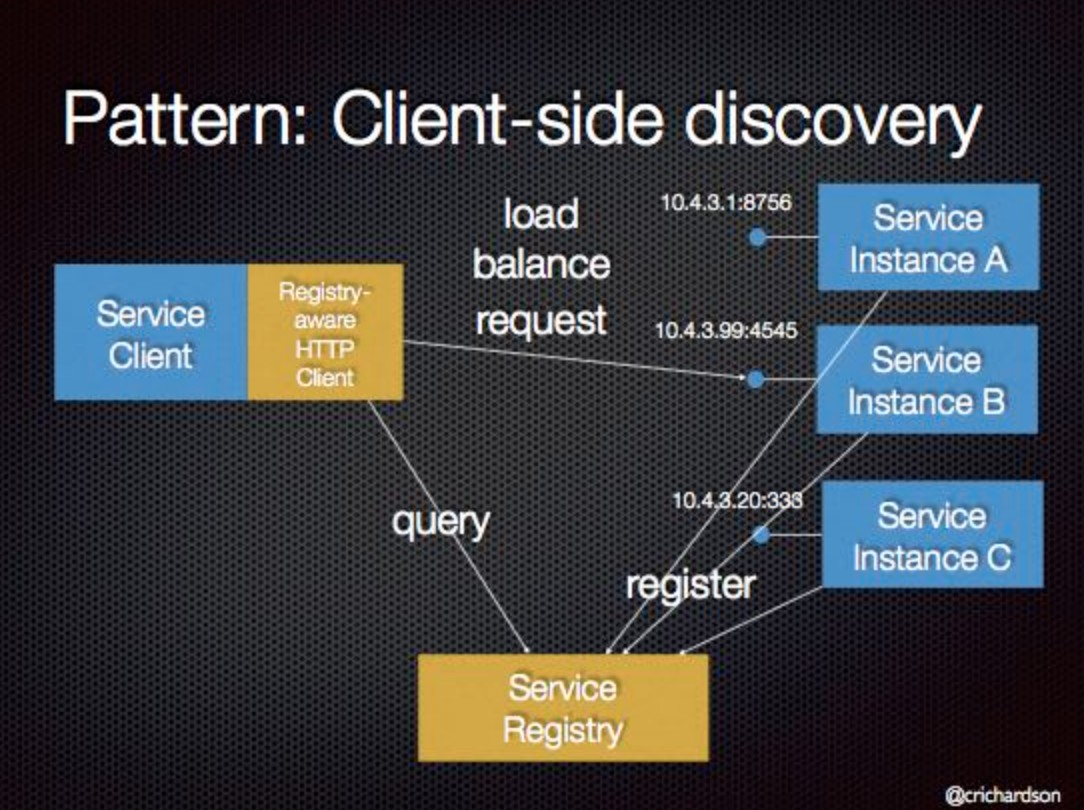
\includegraphics[width=1\textwidth]{resources/chapter-2/client-side-discovery.jpg}
  \caption{Visualisasi \textit{Client Side Discovery} \parencite{clientsidediscovery} }
  \label{fig:client-side-discovery}
\end{figure}

\subsection{\textit{Self Registration}}
\textit{Pattern self registration service discovery} merupakan \textit{pattern} yang mudah untuk dilakukan. Pada dasarnya \textit{pattern} ini mirip dengan \textit{3rd party registration} yaitu sistem akan meregister \textit{service} ketika service dinyalakan dan \textit{service} akan di-\textit{unregister} ketika dimatikan. Meskipun solusi ini sederhana namun terdapat dua halangan diantaranya

\begin{enumerate}
  \item \textit{service} yang \textit{crash} harus dapat di-\textit{unregister} dari \textit{registry}
  \item \textit{service} yang sedang tidak bisa melayani permintaan harus di-\textit{unregister} dari \textit{registry} untuk menghindari terjadinya \textit{crash}
\end{enumerate}

Selain itu \textit{client} juga harus melakukan poling untuk mendapatkan data terbaru \textit{service} yang sedang aktif dan dapat menerima permintaan \parencite{selfregistration}.

\subsection{\textit{Server-side}}
Solusi ini memiliki visualisasi yang sama dengan \textit{client side discovery} pada \textbf{Gambar \ref{fig:client-side-discovery}}. Perbedaan yang mencolok yaitu alih alih \textit{client} yang melakukan request ke \textit{service registry}, \textit{client} akan melakukan \textit{request} kepada \textit{load balancer} dan \textit{load balancer} lah yang akan melakukan pencarian layanan mana yang sedang aktif dan dapat menerima permintaan. Cara ini merupakan cara yang paling umum digunakan untuk melakukan \textit{scaling} pada \textit{service} \parencite{servicesidediscovery}.


% \section{Penelitian dan Riset Terkait}
\label{sec:riset-terkait}
Berikut adalah beberapa penelitian dan riset yang pernah dilakukan sebelumnya dan berhubungan dengan tugas akhir ini.

\subsection{\textit{Large-Scale Provisioning of
    Resource Constrained
    IoT Deployments, LEONORE}}
\label{subsec:leonore}

Riset ini menjelaskan mengenai cara pembuatan sebuah infrastruktur untuk melakukan \textit{provisioning} perangkat IoT dalam skala besar. Penelitian ini berfokus untuk membuat sebuah pendekatan terstruktur dalam menyediakan layanan \textit{deployment} lingkungan IoT dengan dua metode, yaitu \textit{Push} dan \textit{Pull}.

LEONORE dibuat untuk menyelesaikan tantangan, yaitu mengelola jutaan perangkat IoT yang heterogen pada sistem skala besar yang memiliki domain \textit{smart city}. Solusi yang sudah ada sering kali bersifat \textit{partial} ataupun manual dalam menangani sebagian infrastruktur. Tentunya, Hal ini tidak efisien dan mahal karena membutuhkan banyak tenaga kerja. Oleh karena itu, LEONORE menghadirkan solusi provisioning yang skalabel dan elastis untuk mengelola perubahan dan kebutuhan baru.

Arsitektur LEONORE dibuat dengan membuat 4 API yang dapat diakses oleh mulai dari  \textit{User API, Repository API, Device API, serta Provisioning}. Arsitektur ini memilki cara kerja yaitu menyimpan seluruh \textit{image} atau dapat disebut sebagai \textit{deployment plan} pada \textit{repository}, apabila \textit{repository} membutuhkan \textit{dependency} lain maka akan diletakan pada bagian \textit{artifact}. \textit{Artifact} dibuat dan diproses oleh \textit{package builder} yang seluruh \textit{resources}-nya diatur oleh komponen manajemen yaitu \textit{package, dependency management} serta \textit{gateway management}. Setelah siap untuk di-\textit{deploy}, bagian IoT\textit{gateway handler} melakukan \textit{provisioning} kepada target \textit{device}. Secara umum, arsitektur LEONORE dapat dilihat pada gambar \ref{fig:arsitektur-leonore}.

\begin{figure}[ht]
  \centering
  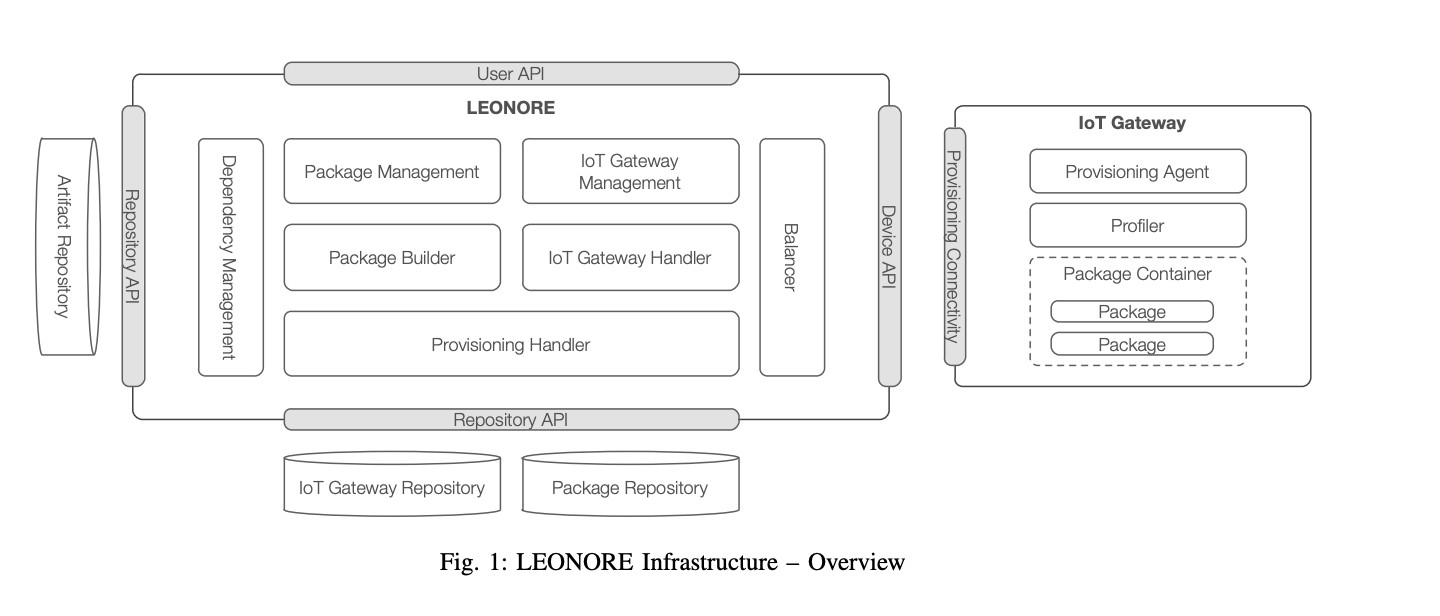
\includegraphics[width=0.8\textwidth]{resources/chapter-2/arsitektur-leonore.jpg}
  \caption{Arsitektur Leonore \parencite{vogler2015leonore}}
  \label{fig:arsitektur-leonore}
\end{figure}

Ilustrasi cara kerja LEONORE dapat dilihat pada gambar \ref{fig:sequence-leonore}. Berikut adalah cara kerja dari sistem LEONORE:
\begin{enumerate}
  \item Mengecek ketersediaan \textit{Artifact}.
  \item Mengambil \textit{Iot Gateway} sebagai grup yang akan di-\textit{deploy}.
  \item Mendelegasikan tugas \textit{deployment} ke setiap \textit{Gateway} IoT.
  \item Analisa kompatibilitas untuk setiap \textit{nodes}.
  \item Resolve \textit{dependency} dan membuat \textit{application package} sesuai dengan grup \textit{Gateway} IoT
  \item Menjalankan \textit{provisioning}
  \item Menunggu hingga setiap \textit{nodes} selesai lalu melakukan pengecekan untuk setiap \textit{nodes} hingga proses selesai
\end{enumerate}

\begin{figure}[ht]
  \centering
  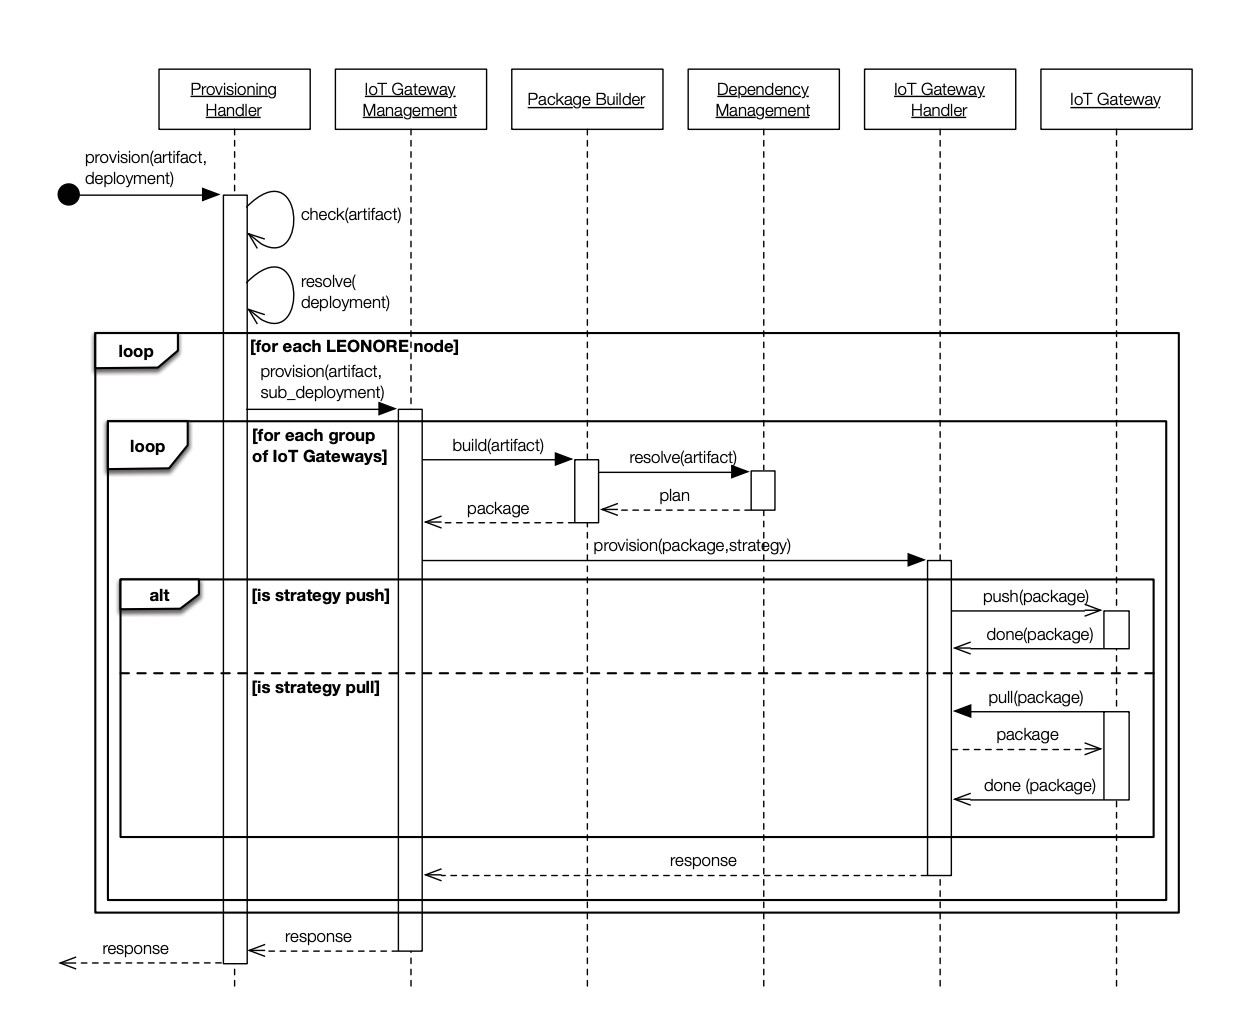
\includegraphics[width=0.8\textwidth]{resources/chapter-2/leonore-sequence.jpg}
  \caption{Sequence Diagram Proses \textit{Deployment} LEONORE \parencite{vogler2015leonore}}
  \label{fig:sequence-leonore}
\end{figure}

Untuk mengevaluasi kinerja LEONORE, dilakukan pengujian pada \textit{cloud} berisi 1000 perangkat yang divirtualisasi menggunakan \textit{docker}. Hasilnya, LEONORE dapat melakukan \textit{provisioning} seluruh perangkat dengan waktu yang \textit{reasonable}. Metode \textit{pull provisioning} menghasilkan latensi yang tinggi apabila dibandingkan dengan metode \textit{push} yang memberikan hasil cukup baik.
\subsection{DIANE – Dynamic IoT Application Deployment}
\textit{DIANE} merupakan penelitian lanjutan dari LEONORE yang telah dijelaskan pada bagian \ref{subsec:leonore}. DIANE adalah sebuah sistem ataupun \textit{framework} yang dapat menghasilkan topologi \textit{deployment} secara dinamis yang dioptimalkan untuk aplikasi IoT serta disesuaikan dengan infrastruktur terkait.

Berbeda dengan LEONORE, DIANE tidak menggunakan \textit{application package}, melainkan menggunakan model deklaratif berbasis \textit{resource} dari \textit{aplikasi} yang dibuat. Pendekatan ini memungkinkan penyediaan komponen aplikasi yang fleksibel pada infrastruktur \textit{cloud} serta \textit{gateway} IoT \parencite{vogler2015diane}. DIANE menggunakan \textit{Methodology for Architecture and Deployment of Cloud Application Topologie} (MADCAT) untuk mendefinisikan komponen yang digunakan. Pada metode ini, terdapat dua unit yang menjadi komponen penting pada sistem, yaitu \textit{Technical Unit}(TU) serta \textit{Deployment Unit}(DU) \parencite{madcat}. TU berikatan dengan aplikasi yang ingin dibuat sehingga satu \textit{TU} dapat memiliki satu atau lebih \textit{DU} yang mendefinisikan proses \textit{deployment} yang dibuat. Ilustrasi TU dan DU dapat dilihat pada gambar \ref{fig:diane-tu} dan \ref{fig:diane-du}.

\begin{figure}[ht]
  \centering
  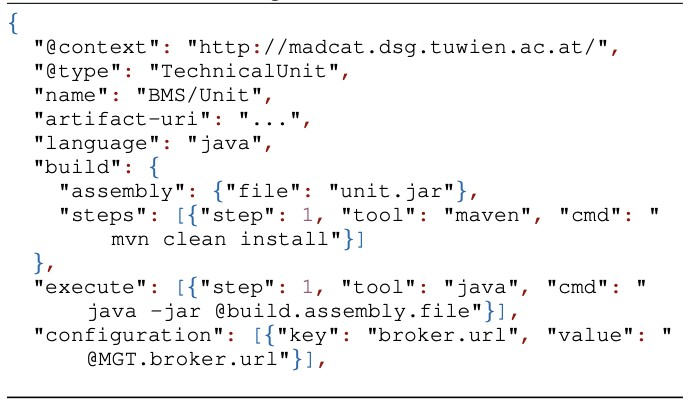
\includegraphics[width=0.8\textwidth]{resources/chapter-2/diane-technical-unit.jpg}
  \caption{\textit{Technical Unit} DIANE \parencite{vogler2015diane}}
  \label{fig:diane-tu}
\end{figure}

\begin{figure}[ht]
  \centering
  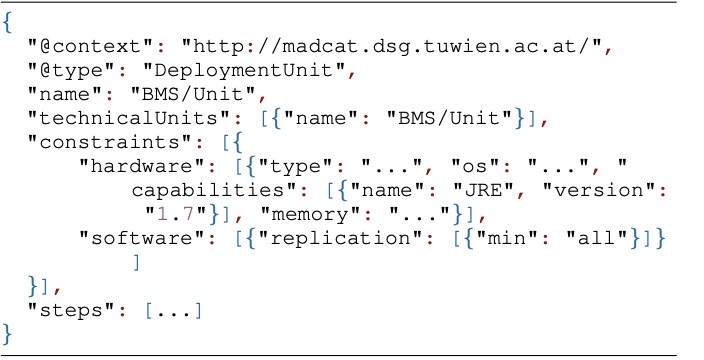
\includegraphics[width=0.8\textwidth]{resources/chapter-2/diane-deployment-unit.jpg}
  \caption{\textit{Deployment Unit} DIANE \parencite{vogler2015diane}}
  \label{fig:diane-du}
\end{figure}

DIANE memiliki arsitektur yang terdiri dari \textit{Deployment Registry}, \textit{Deployment Handler}, \textit{Artifact Management}, \textit{Deployment Generator}, \textit{Dependency Management}, dan \textit{Constraint Handler}. Setelah seluruh proses dilewati, DIANE akan berinteraksi dengan \textit{Service API} untuk melakukan \textit{provisioning} dengan LEONORE. Ilustrasi arsitektur DIANE dapat dilihat pada gambar \ref{fig:diane-arch}.

\begin{figure}[ht]
  \centering
  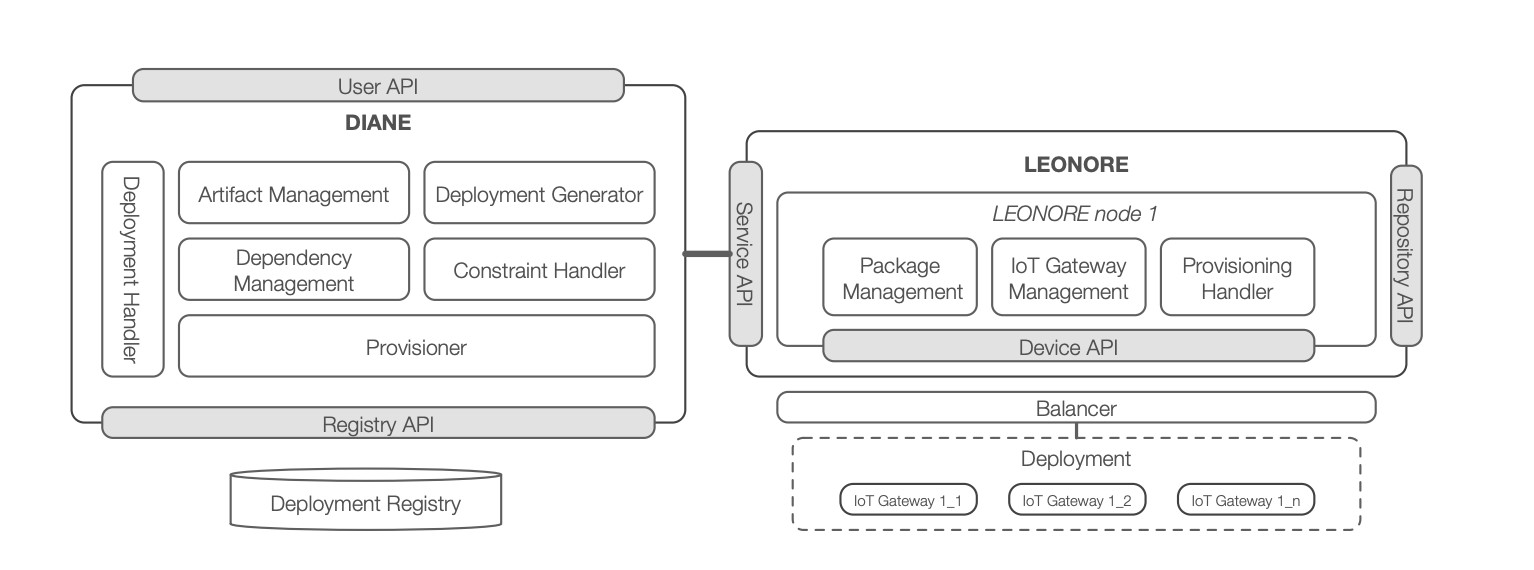
\includegraphics[width=0.8\textwidth]{resources/chapter-2/diane-architecture.jpg}
  \caption{Arsitektur DIANE \parencite{vogler2015diane}}
  \label{fig:diane-arch}
\end{figure}

\subsection{China Electronic Toll Colleciton}
China memiliki masyarakat yang sangat banyak dan setiap masyarakat memiliki sekurang-kurangnya satu kendaraan. Seiring dengan bertambahnya jumlah masyarakat di China, jalanan yang ada di China semakin penuh dengan kendaraan yang sehingga menghasilkan kemacetan terutama pada tol bagian pembayaran. Untuk mengatasi masalah ini, China menggunakan \textit{Electronic Toll Colleciton} (ETC) yang di integrasikan dengan setiap kendaraan untuk mempercepat proses ini \parencite{penelitianterkait1}. Arsitektur dapat dilihat pada \ref{fig:china-highways}.

\begin{figure}[ht]
  \centering
  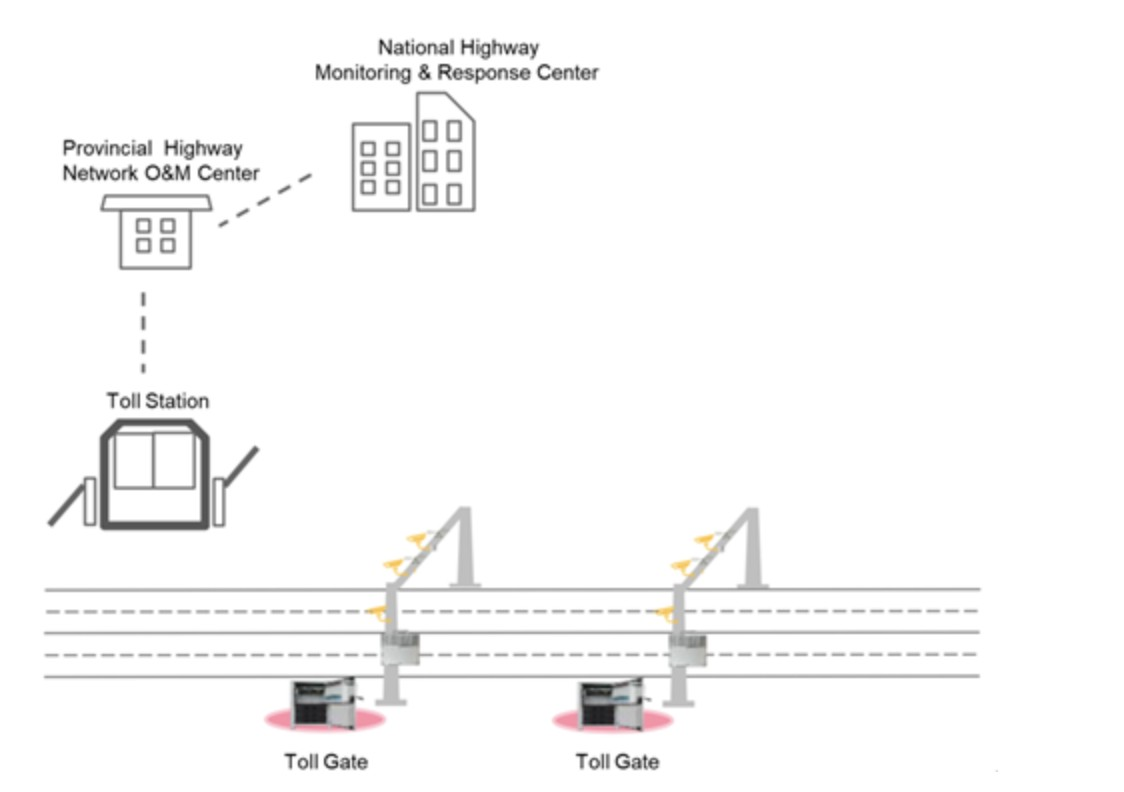
\includegraphics[width=0.8\textwidth]{resources/chapter-2/china-highways.jpg}
  \caption{Implementasi Sistem \textit{ETC} di China \parencite{penelitianterkait1}}
  \label{fig:china-highways}
\end{figure}

China menggunakan KubeEdge untuk melakukan proses \textit{deployment} ETC untuk 100,000 \textit{nodes} dengan total 500,000 aplikasi yang diluncurkan menggunakan KubeEdge tersebar untuk 29 dari 34 provinsi. Proses \textit{deployment} dilakukan secara otomatis dengan membuat sistem \textit{workflow engine} pada Kubernetes sehingga proses \textit{deployment} dapat dilakukan dengan cepat dan mudah. Dengan menggunakan metode ini, sistem pembayaran tol di China menjadi 10x lebih cepat dari sebelumnya \parencite{penelitianterkait1}. Gambar dapat dilihat pada \ref{fig:architecture-china-highways}.

\begin{figure}[ht]
  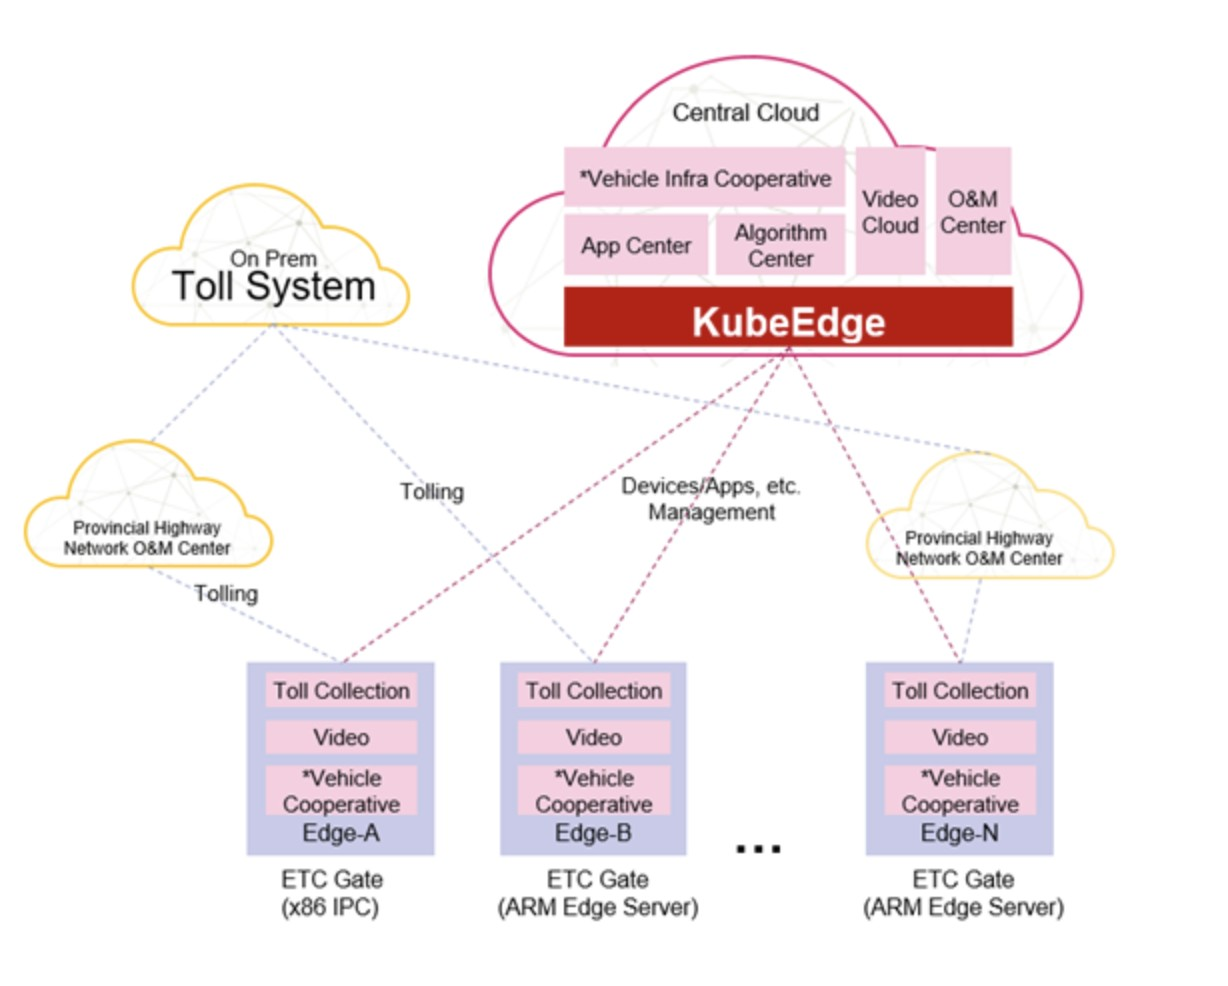
\includegraphics[width=0.8\textwidth]{resources/chapter-2/arsitektur-china-highways.jpg}
  \caption{Arsitektur Sistem \textit{ETC} di China \parencite{penelitianterkait1}}
  \label{fig:architecture-china-highways}
\end{figure}
\subsection{A Model for the Remote Deployment, Update, and Safe Recovery for Commercial Sensor-Based IoT Systems}
Penelitian ini menggali tantangan-tantangan khusus terkait infrastruktur yang didedikasikan untuk penyebaran dan manajemen aplikasi secara jarak jauh. Penelitian ini membahas tantangan-tantangan manajemen terkait sistem sensor IoT dan mengusulkan sebuah cara serta metodologi untuk mengatasi hal tersebut.

Penelitian ini mengimplementasikan solusi sebagai sistem infrastruktur perangkat lunak untuk produk IoT bisnis yang lengkap. Penelitian ini melakukan \textit{deployment} pada 100 perangkat penjual minuman yang tersebar di tiga lokasi. Setiap perangkat bergantung pada sensor yang memantau statusnya dan pada \textit{gateway} yang mengendalikan perilakunya. Arsitektur sistem dapat dilihat pada gambar \ref{fig:architecture-remote-deployments}.

\begin{figure}[ht]
  \centering
  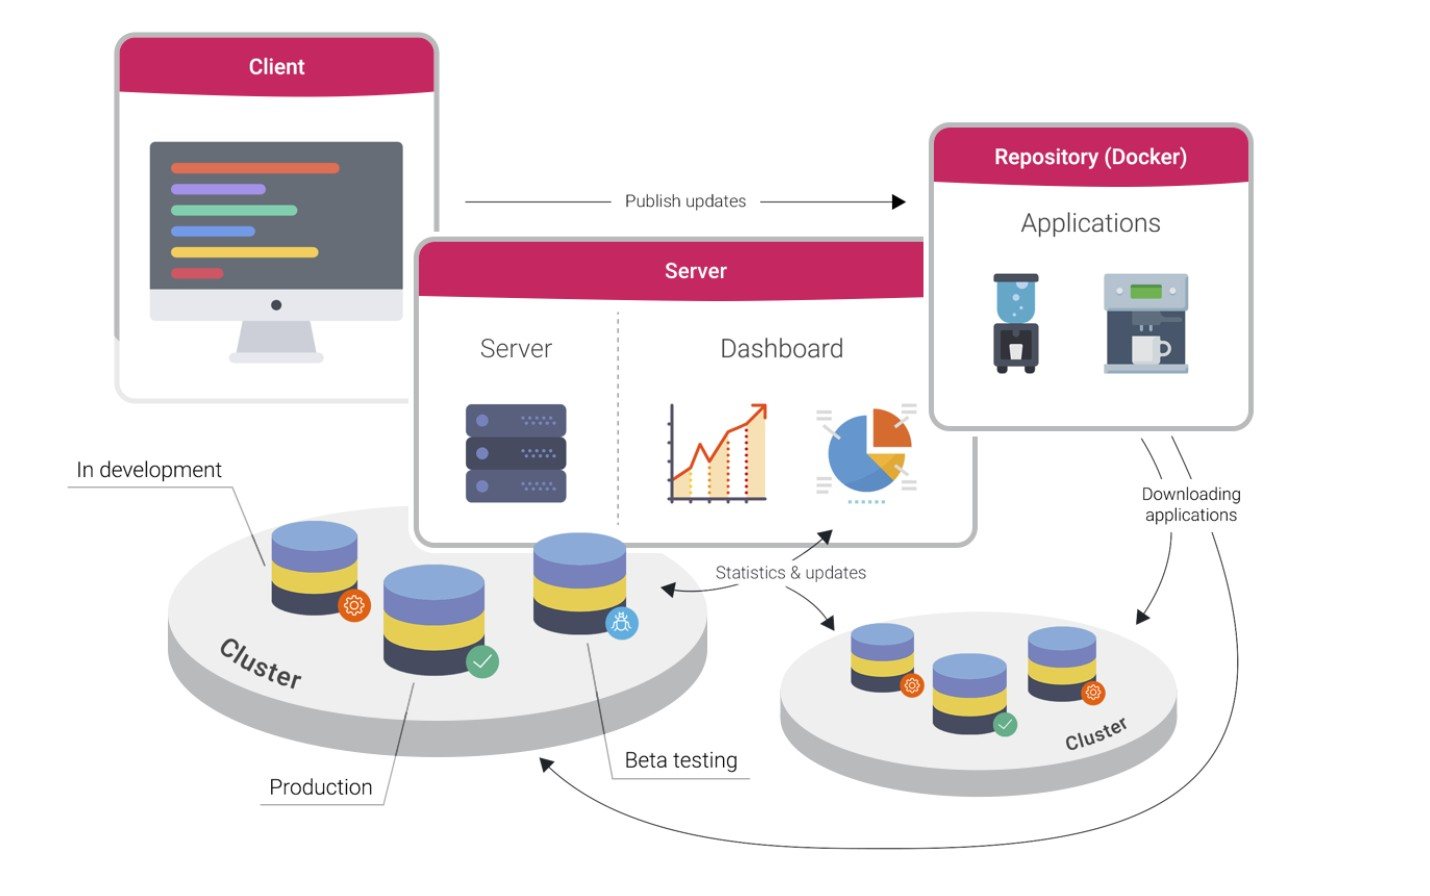
\includegraphics[width=0.8\textwidth]{resources/chapter-2/arsitektur-remote-deployment.jpg}
  \caption{Arsitektur Remote \textit{Deployment} \parencite{RemoteDeployment}}
  \label{fig:architecture-remote-deployments}
\end{figure}

Selama penelitian ini berlangsung, penelitian ini berhasil menerima 133 \textit{update} pada perangkat IoT. 80\% perangkat beroperasi tanpa gangguan selama 250 hari. Sedangkan, 20\% mengalami kegagalan akibat faktor eksternal. Dari 80\% tersebut, 30\% mengalami kegagalan pembaruan sementara akibat kapabilitas perangkat yang berkurang \parencite{RemoteDeployment}.

Solusi yang dibuat penelitian ini mengandalkan keamanan serta \textit{failsafe} yang dapat melakukan \textit{remote deployment} dengan baik serta aman sehingga dapat mendeteksi kegagalan yang terjadi pada perangkat dan melakukan \textit{recovery} dengan cepat. Berikut merupakan beberapa cara untuk melakukan \textit{remote deployment} atau seringkali disebut sebagai OTA \textit{(Over the air)}.

\begin{figure}[ht]
  \centering
  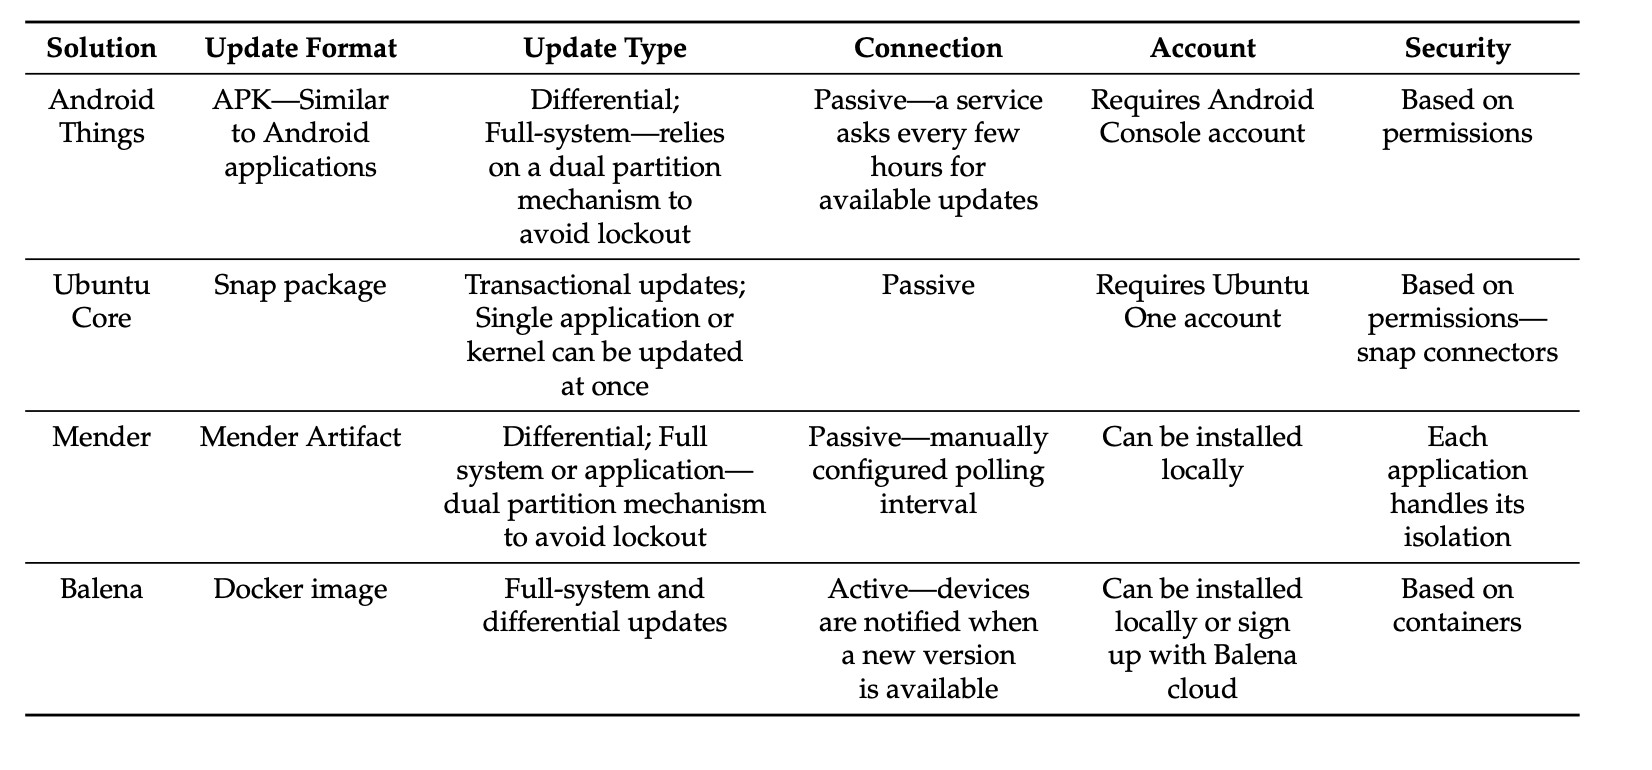
\includegraphics[width=0.8\textwidth]{resources/chapter-2/perbandingan-remote-deployment.jpg}
  \caption{Perbandingan Tata Cara \textit{Remote Deployment} \parencite{RemoteDeployment}}
  \label{fig:comparison-remote-deployments}
\end{figure}

Dapat dilihat dari gambar \ref{fig:comparison-remote-deployments} bahwa terdapat berbagai solusi untuk berbagai tipe \textit{remote deployment}. Pada kasus ini, dapat dibuat suatu cara yang mengadopsi \textit{update type} serta koneksi dari keempat tipe tersebut. Perangkat melakukan \textit{polling} kepada \textit{server} untuk mengecek apakah terdapat versi terbaru atau tidak. Selain itu, dari sisi \textit{Server} juga dapat membuat suatu notifikasi yang dapat diterima oleh perangkat jika terdapat \textit{update} baru yang siap digunakan.